\section{Step 2: Splits}\label{sec:splits}

\emph{What a random split hides.} Table~\ref{tab:perclass} gives per-class F1 for the decision tree on CIC-IoT2023. Macro-F1 is 0.869 (host-pair CI [0.735, 0.877]) under the random split and 0.731 ([0.577, 0.823]) under the temporal split, with Benign FPR 1.1\% and 3.9\%. Two classes are tiny on the temporal test set (Mirai 10 and MITM-ARP 25 flows); macro-F1 over the classes with at least 50 test flows is 0.814. The host-pair intervals overlap substantially, so the macro-F1 gap is not statistically robust: it rests on a few host pairs, mainly the brute-force ones.

\begin{table}[t]
\centering
\caption{Per-class F1 of the decision tree. $n$ is the temporal test support.}
\label{tab:perclass}
\footnotesize
\begin{tabular}{lrcc}
\hline
Class & $n$ & F1 random & F1 temporal \\
\hline
Benign     &  52,993 & 0.99 & 0.97 \\
BruteForce &     605 & 0.99 & 0.10 \\
DDoS-SYN   & 153,402 & 1.00 & 1.00 \\
DoS-HTTP   &  10,110 & 0.99 & 0.92 \\
MITM-ARP   &      25 & 0.11 & 0.02 \\
Mirai      &      10 & 1.00 & 0.95 \\
Recon      &  39,819 & 1.00 & 1.00 \\
Web        &     192 & 0.87 & 0.89 \\
\hline
Macro-F1   & 257,156 & 0.869 & 0.731 \\
\hline
\end{tabular}
\end{table}

\begin{figure}[t]
\centering
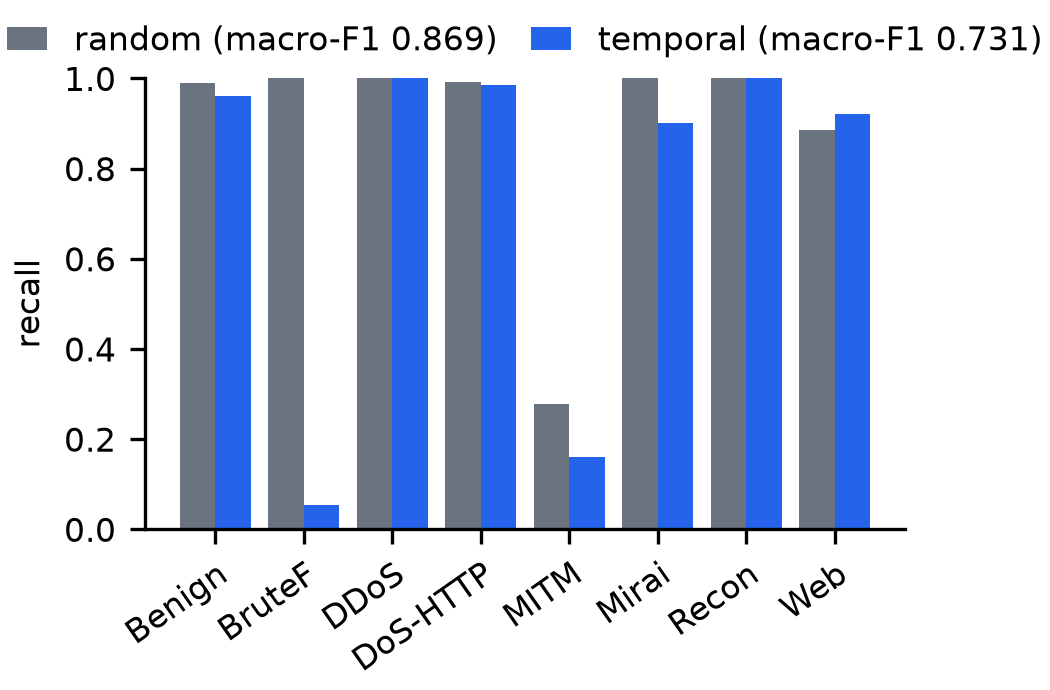
\includegraphics[width=\columnwidth]{../docs/figures/split_recall.png}
\caption{Per-class recall of the decision tree under the random and the temporal split (test support in Table~\ref{tab:perclass}). Brute-force recall falls from 1.00 to 0.05.}
\label{fig:split}
\end{figure}

\emph{A change of attack target.} Fig.~\ref{fig:split} locates the gap: BruteForce recall falls from 1.00 to 0.05. The capture explains why. Its training period contains SSH brute force against .67:22 (13:21--13:43); its test period contains RTSP brute force against two cameras, .11 and .140 on port 554 (13:43--15:01). A random split puts RTSP flows into training and hides that the model learned one service, not ``brute force''. This is a change of target within one capture session, a case of the ``blindness'' that Rasheed and Alobaedy describe under drift~\cite{rasheed2026drift}. It rests on only three host pairs (one SSH pair in training, two RTSP pairs in the test period): under the host-pair bootstrap, temporal BruteForce recall is 0.053 [0.000, 0.842] (random: 1.000 [1.000, 1.000]). We therefore present it as a mechanism shown in a case study, not as a statistically robust effect. The other small classes are similarly uncertain (temporal Mirai 0.90 [0.571, 1.000], 6 pairs; MITM-ARP 0.16 [0.000, 0.375], 13 pairs). The mechanism agrees with IoTGeM's finding that brute-force variants do not generalise~\cite{kostas2024iotgem}.

\emph{Boundary-spanning connections.} A temporal cut by flow start does not cut connections: a long connection yields several flows (active timeout 120\,s). Of the temporal test flows, 36.1\% (92,766 of 257,156) share a 5-tuple with a training flow of the same capture, i.e.\ continue a connection that started in training; we call these connections boundary-spanning. Removing them lowers the deployed tree's macro-F1 from 0.725 to 0.604, mostly because Mirai is then left without test flows; over the seven classes that keep test flows the change is 0.700 to 0.690, concentrated in DoS-HTTP (F1 0.919 to 0.851). All 10 Mirai test flows are such continuations, so the Mirai test score is not evidence of generalisation. The live windows (Section~\ref{sec:live}) exclude these connections.

\emph{What flow features cannot see.} MITM-ARP reaches precision 0.01 and recall 0.16 on the temporal split. An ARP-spoofing flow is a victim's ordinary traffic relayed through the attacker, and the MAC address, the only distinguishing field, is not a model input. Section~\ref{sec:response} covers this class with an ARP rule.

\begin{table}[t]
\centering
\caption{IoT-23, deployed tree trained on Zeek labels. Common: macro-F1 over the four classes present in both halves of both splits. Spanning: share of boundary-spanning test flows.}
\label{tab:iot23split}
\footnotesize
\setlength{\tabcolsep}{2.5pt}
\begin{tabular}{lccccc}
\hline
Split & Macro-F1 & Flow CI & Host-pair CI & Common & Spanning \\
\hline
Temporal   & 0.649 & [0.648, 0.650] & [0.613, 0.655] & 0.973 & 4.1\% \\
Stratified & 0.863 & [0.764, 0.923] & [0.638, 0.939] & 0.956 & 5.8\% \\
\hline
\end{tabular}
\end{table}

\emph{IoT-23: the temporal gap does not replicate.} On IoT-23 the temporal macro-F1 is again lower than the stratified one (Table~\ref{tab:iot23split}), but for a different reason: missing classes. Under the temporal split DDoS has no training flows and FileDownload no test flows, so both score 0 by construction. On the four classes present in both halves (Attack, Benign, C\&C, PortScan), the temporal split scores higher than the stratified one. The stratified macro-F1 in turn rests on 63 DDoS and 2 FileDownload test flows from one or two host pairs each, which is why its host-pair interval is so wide. Flow-level intervals understate uncertainty here too: temporal C\&C, with 7 host pairs, has F1 0.945 with a host-pair CI of [0.731, 0.983] against a flow CI of [0.941, 0.949]. Boundary-spanning flows recur and concentrate in C\&C (36.5\% of its temporal and 68\% of its stratified test flows); without them the stratified macro-F1 falls from 0.863 to 0.809, while the temporal one stays at 0.649. We therefore do not claim that the CIC-IoT2023 temporal gap replicates. What carries over are three requirements for the check: a temporal split must verify that each class is present in both halves, intervals must resample host pairs rather than flows, and the boundary-spanning share must be reported, because it inflates stratified scores.
